\chapter{Исследовательская часть}
В данной части будет проведено исследование процессорного времени выполнения разработанных алгоритмов.

\section{Технические характеристики}
Исследования проводились на устройстве со следующими характеристиками[3]
\begin{itemize}
\itemоперационная система: MacOS Tahoe 26.0.1 (25A362);
\itemпроцессор: Apple M3, 8 ядер;
\itemоперативная память: 16 Гигабайт, LPDDR5;
\end{itemize}	


\section{Реализация замеров}
Во время выполнения замеров устройство было подключено к источнику питанию и не выполняло сторонних процессов. Замеры проводились с помощью встроенной библиотеки $chrono$. Для каждого размера последовательности проводилось 500 запусков для каждого алгоритма, после чего время выполнения усреднялось. Для проведения замеров была отключена оптимизация компилятора флагом -o0[9]. Реализация функции замера времени выполнения приведена на листинге \ref{list:time}
\begin{lstlisting}[language=C++, caption=Функция замера времени выполнения, captionpos=b, label=list:time]
 auto start = std::chrono::high_resolution_clock::now();
for (size_t j = 0; j < EXP_COUNT; j++) {
	max = INT_MIN;
	sequence->recursion_max(max, 0);
}
auto end = std::chrono::high_resolution_clock::now();
auto duration = std::chrono::duration_cast<std::chrono::microseconds>(end-start);

\end{lstlisting}

\section{Оценка времени работы алгоритмов}
Были проведены замеры процессорного времени для реализаций алгоритмов нахождения максимума последовательности с размерами от 0 до 35000. Шаг увелечения размеров для обоих замеров — 1000. 

На рисунках \ref{fig:random}, \ref{fig:straight}, \ref{fig:reverse} продемонстрирована зависимость времени выполнения в зависимости от размера и содержимого последовательности. Итерационная реализация алгоритма в худшем случаее выполняется быстрее в 4.4 раза (рисунок №\ref{fig:straight}) чем рекурсивная, а в лучшем случае в 7 раз (рисунок №\ref{fig:random}). Скорость выполнения реализации алгоритма зависит не только от размера массива, но и от самих данных, которые содержутся в массиве. Если числа отсортированы в порядке возрастания, то каждую итерацию будет обновляться максимум. Напротив, если последовательность отсортирована по убыванию, то значение максимума установится, обновится только 1 раз. Таким образом лучший случай выполняется быстрее в среднем 1.2 раза чем худший.
\begin{figure}[H]
	\centering
	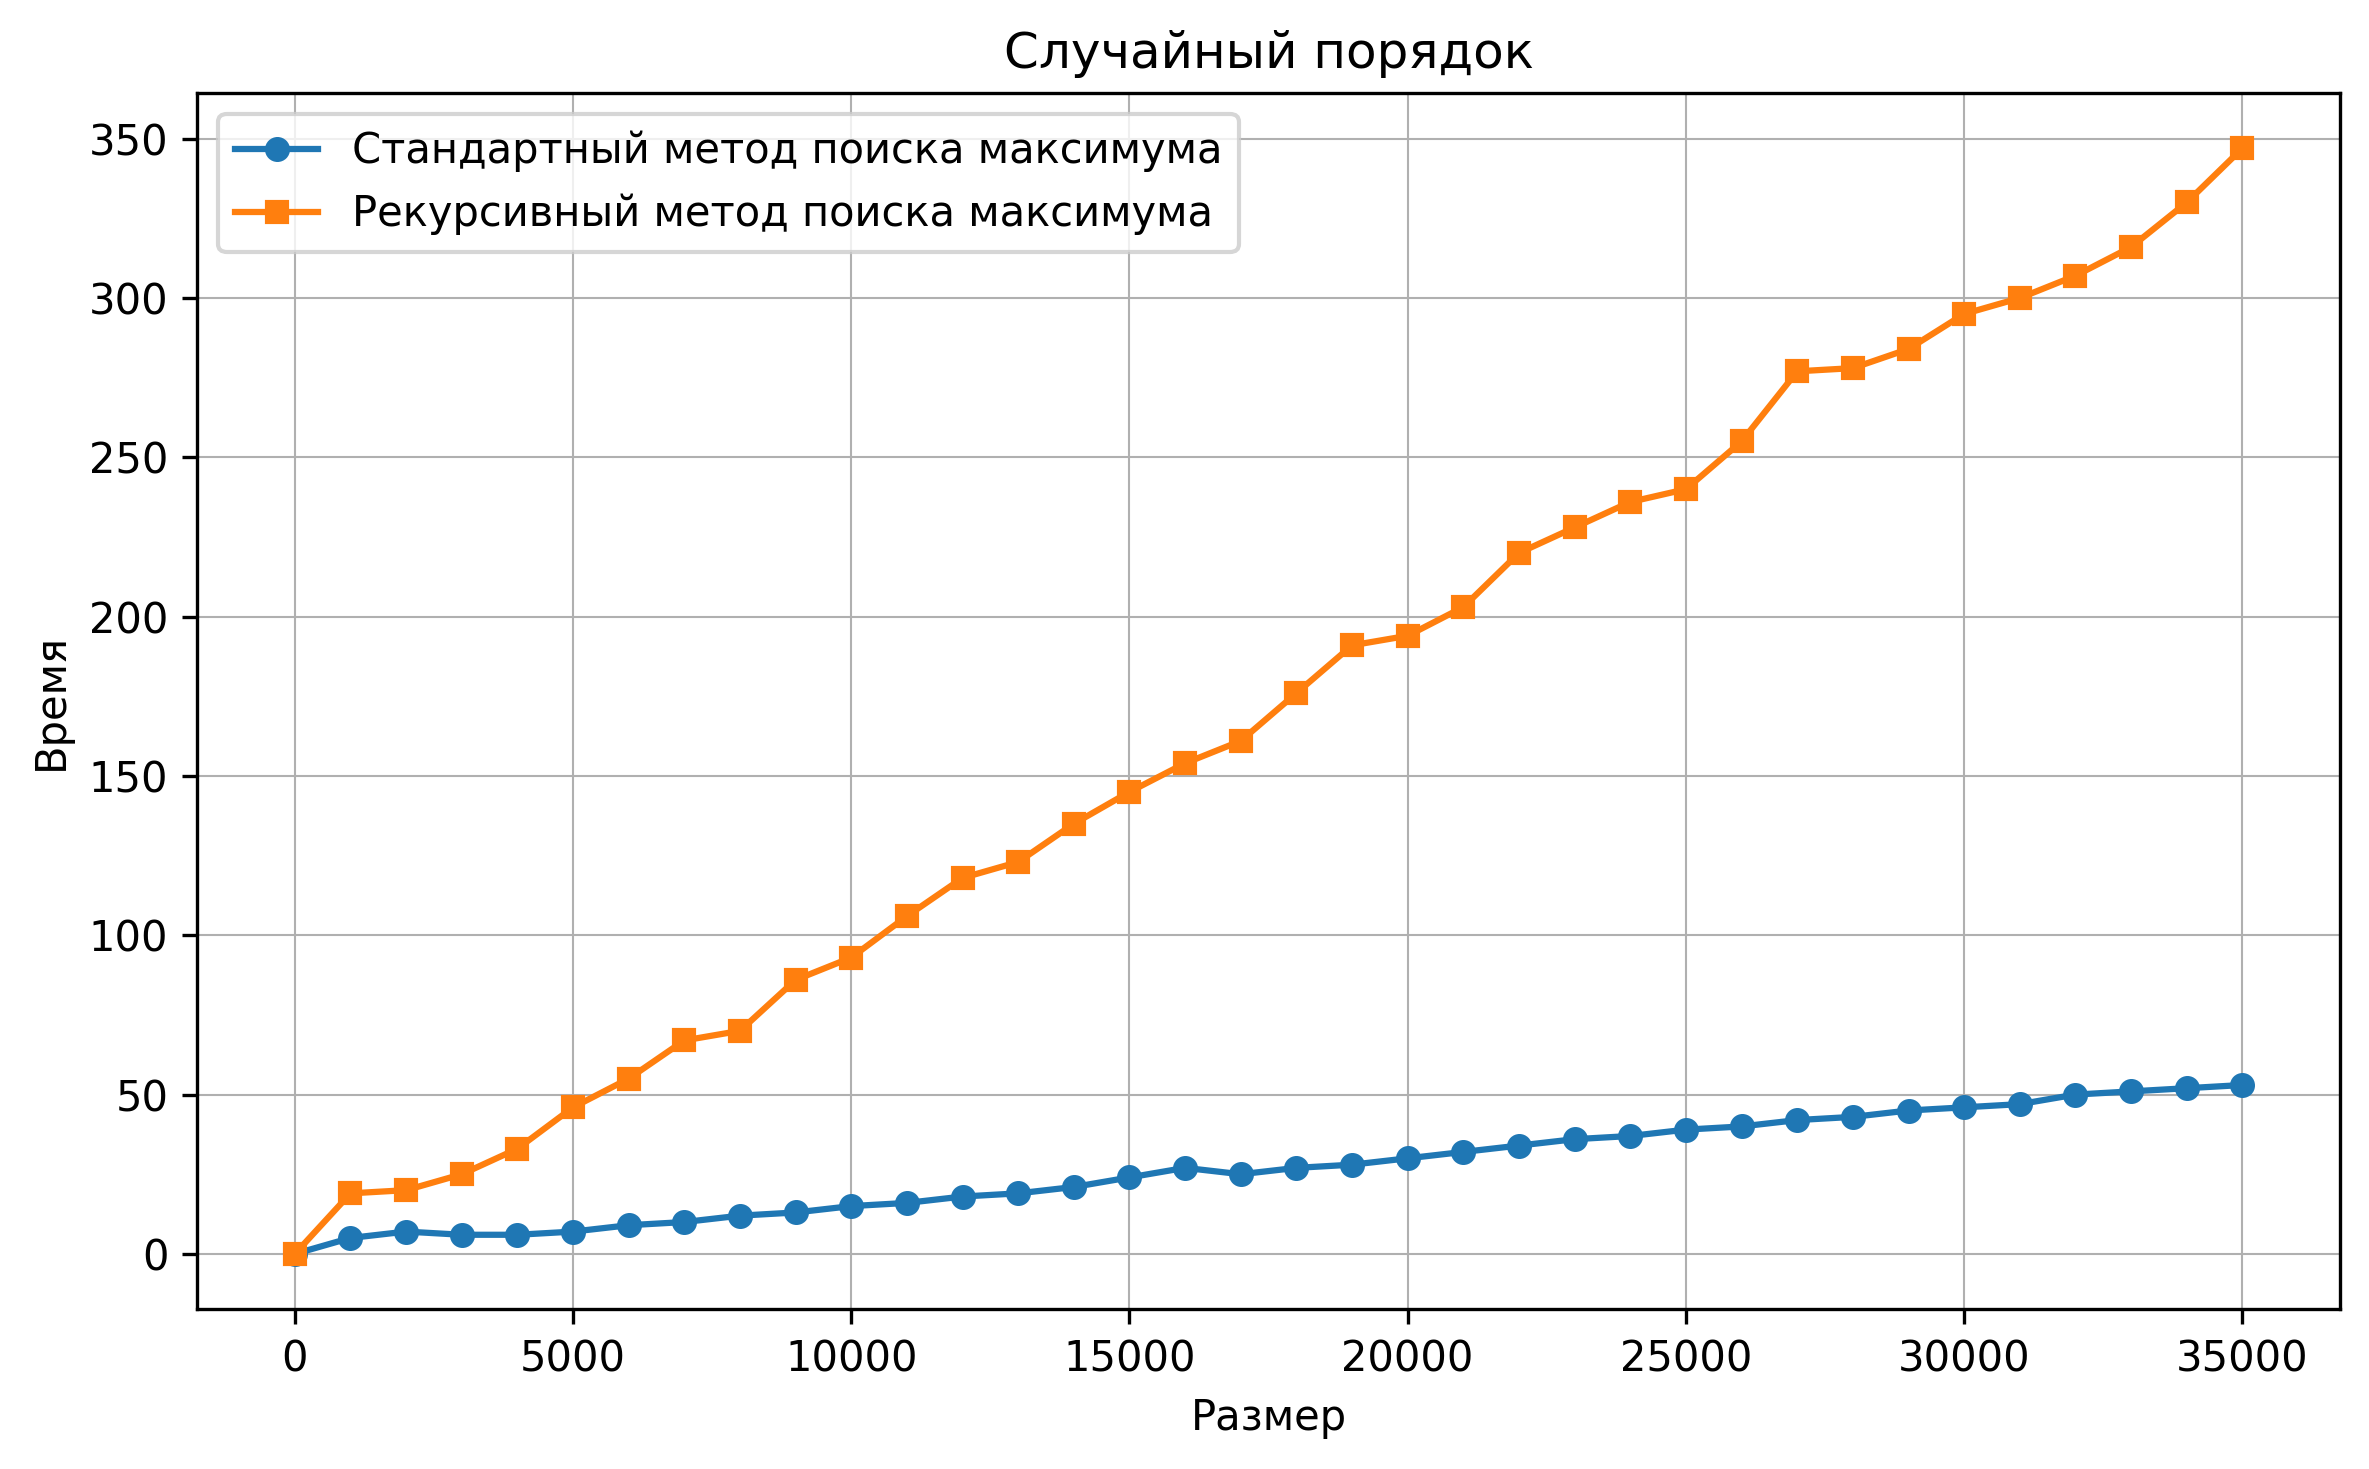
\includegraphics[width=0.9\linewidth]{./images/chart_1.png}
	\caption{Зависимость времени выполнения реализации алгоритма от размера массива, заполненного случайными числами}
	\label{fig:random}
\end{figure}
\begin{figure}[H]
	\centering
	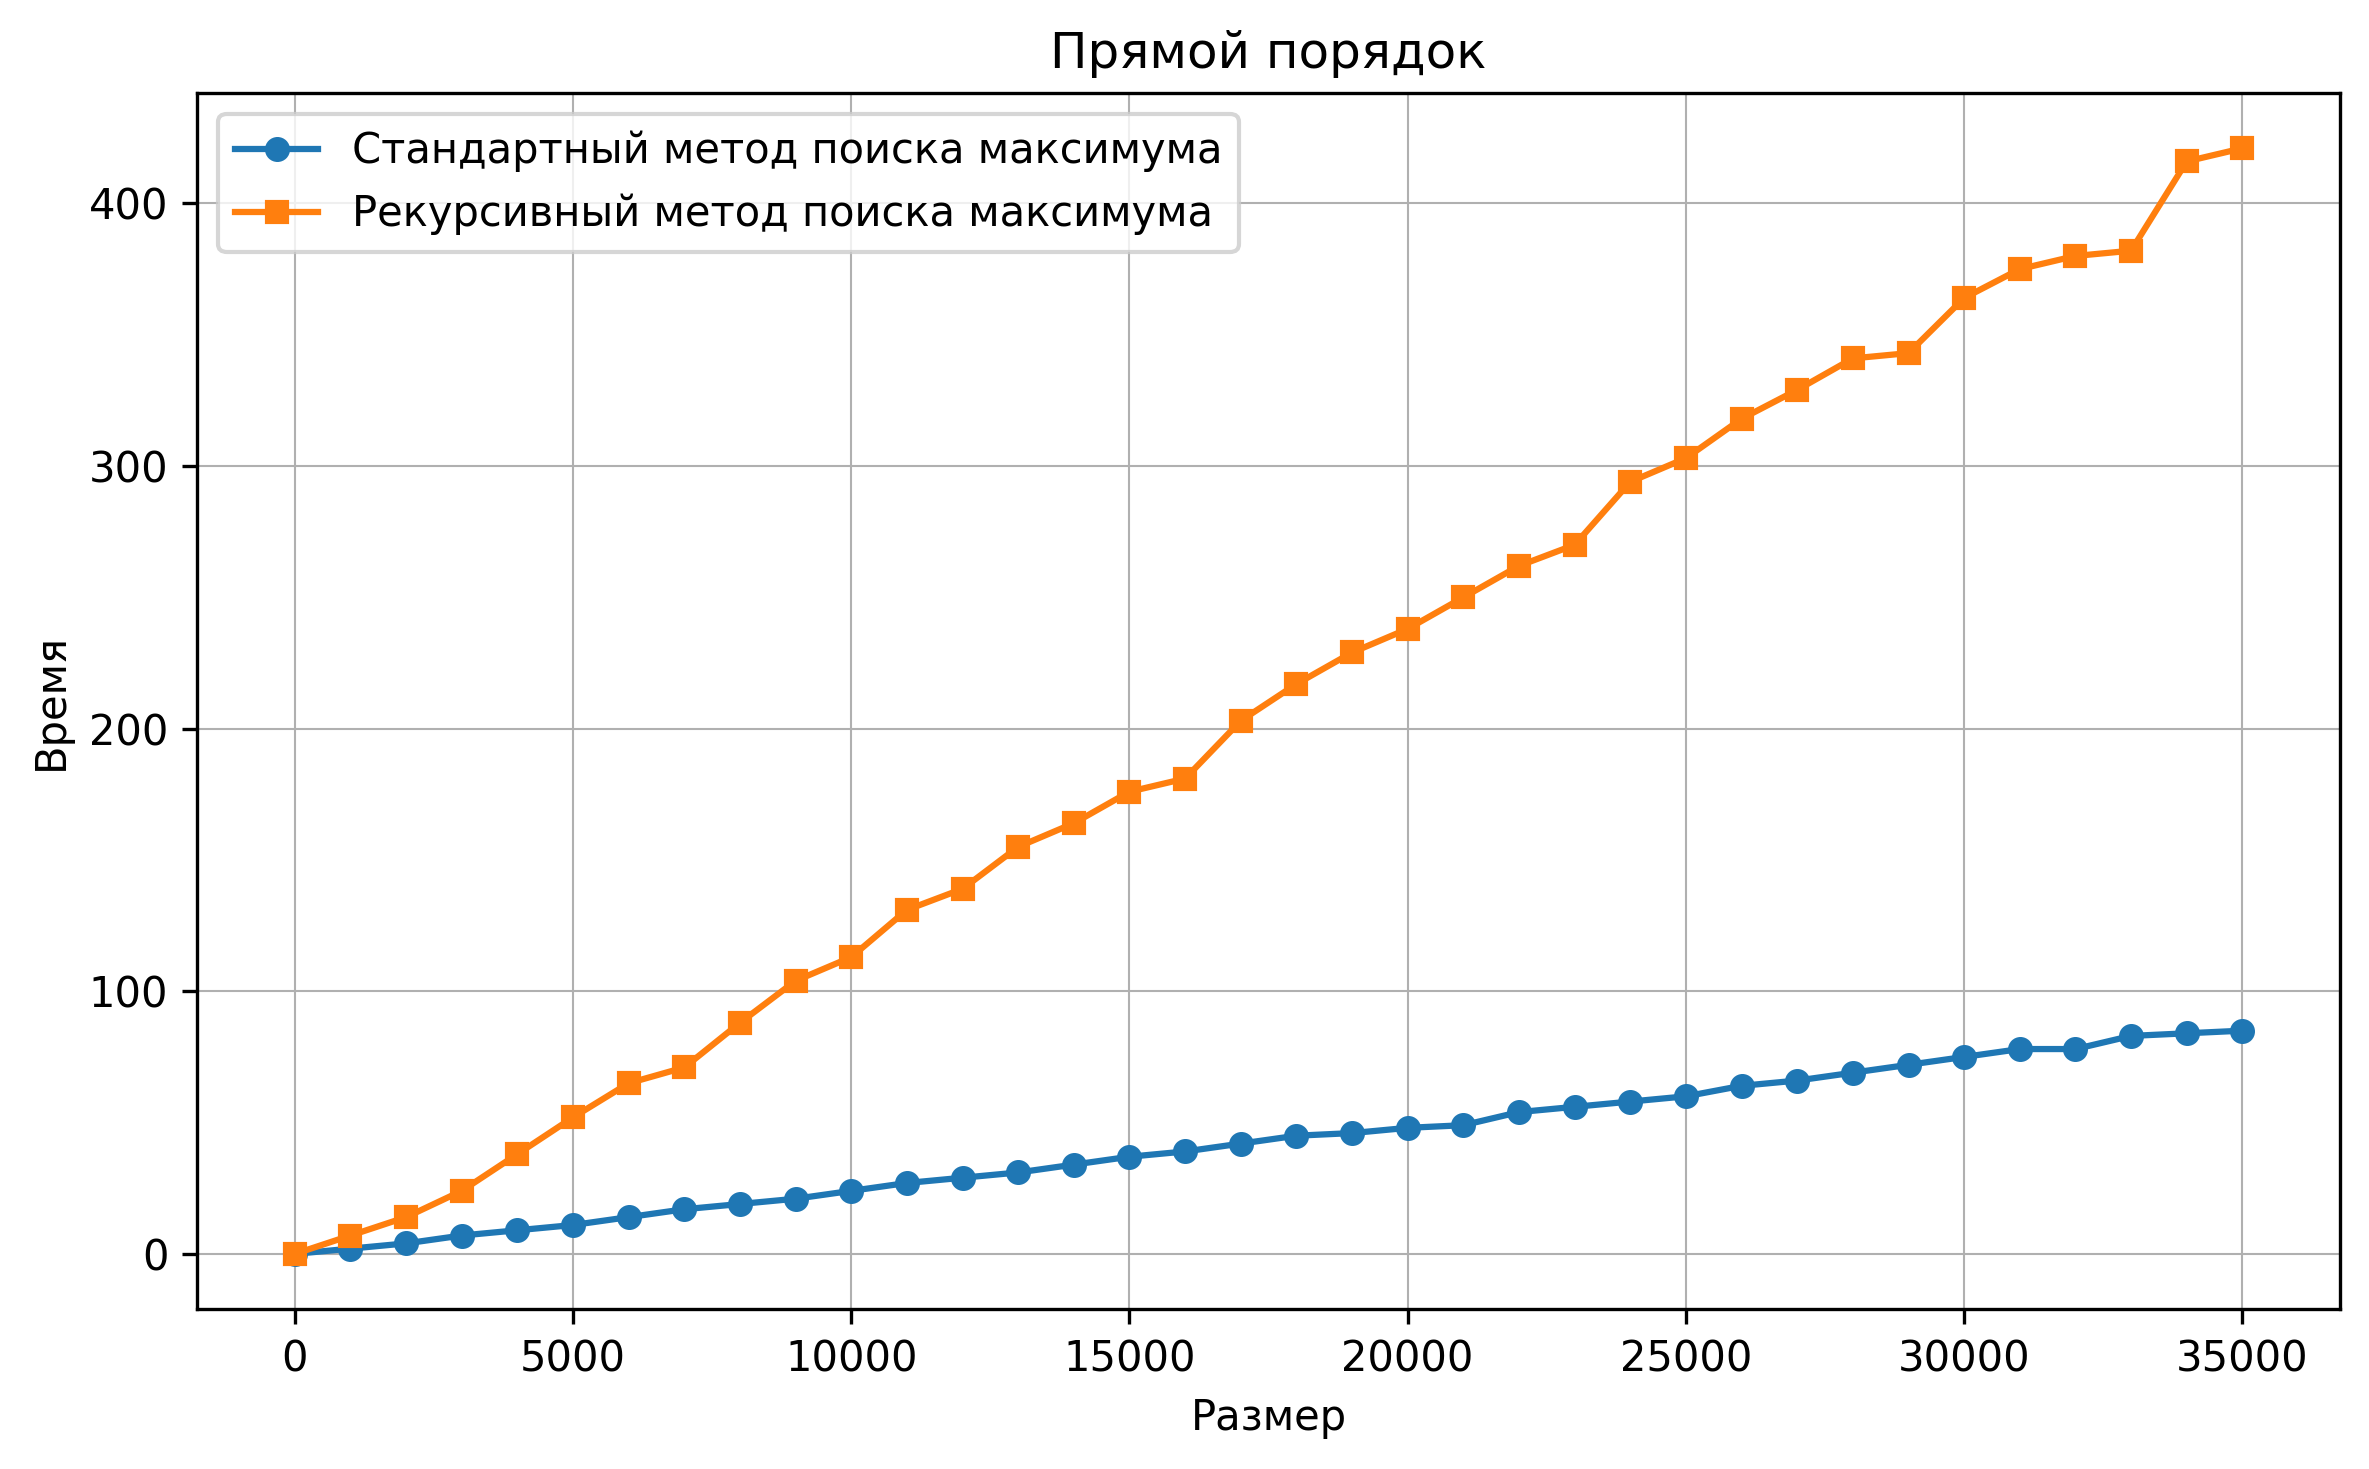
\includegraphics[width=0.9\linewidth]{./images/chart_3.png}
	\caption{Зависимость времени выполнения реализации алгоритма от размера массива, заполненного числами в порядке возрастания}
	\label{fig:straight}
\end{figure}
\begin{figure}[H]
	\centering
	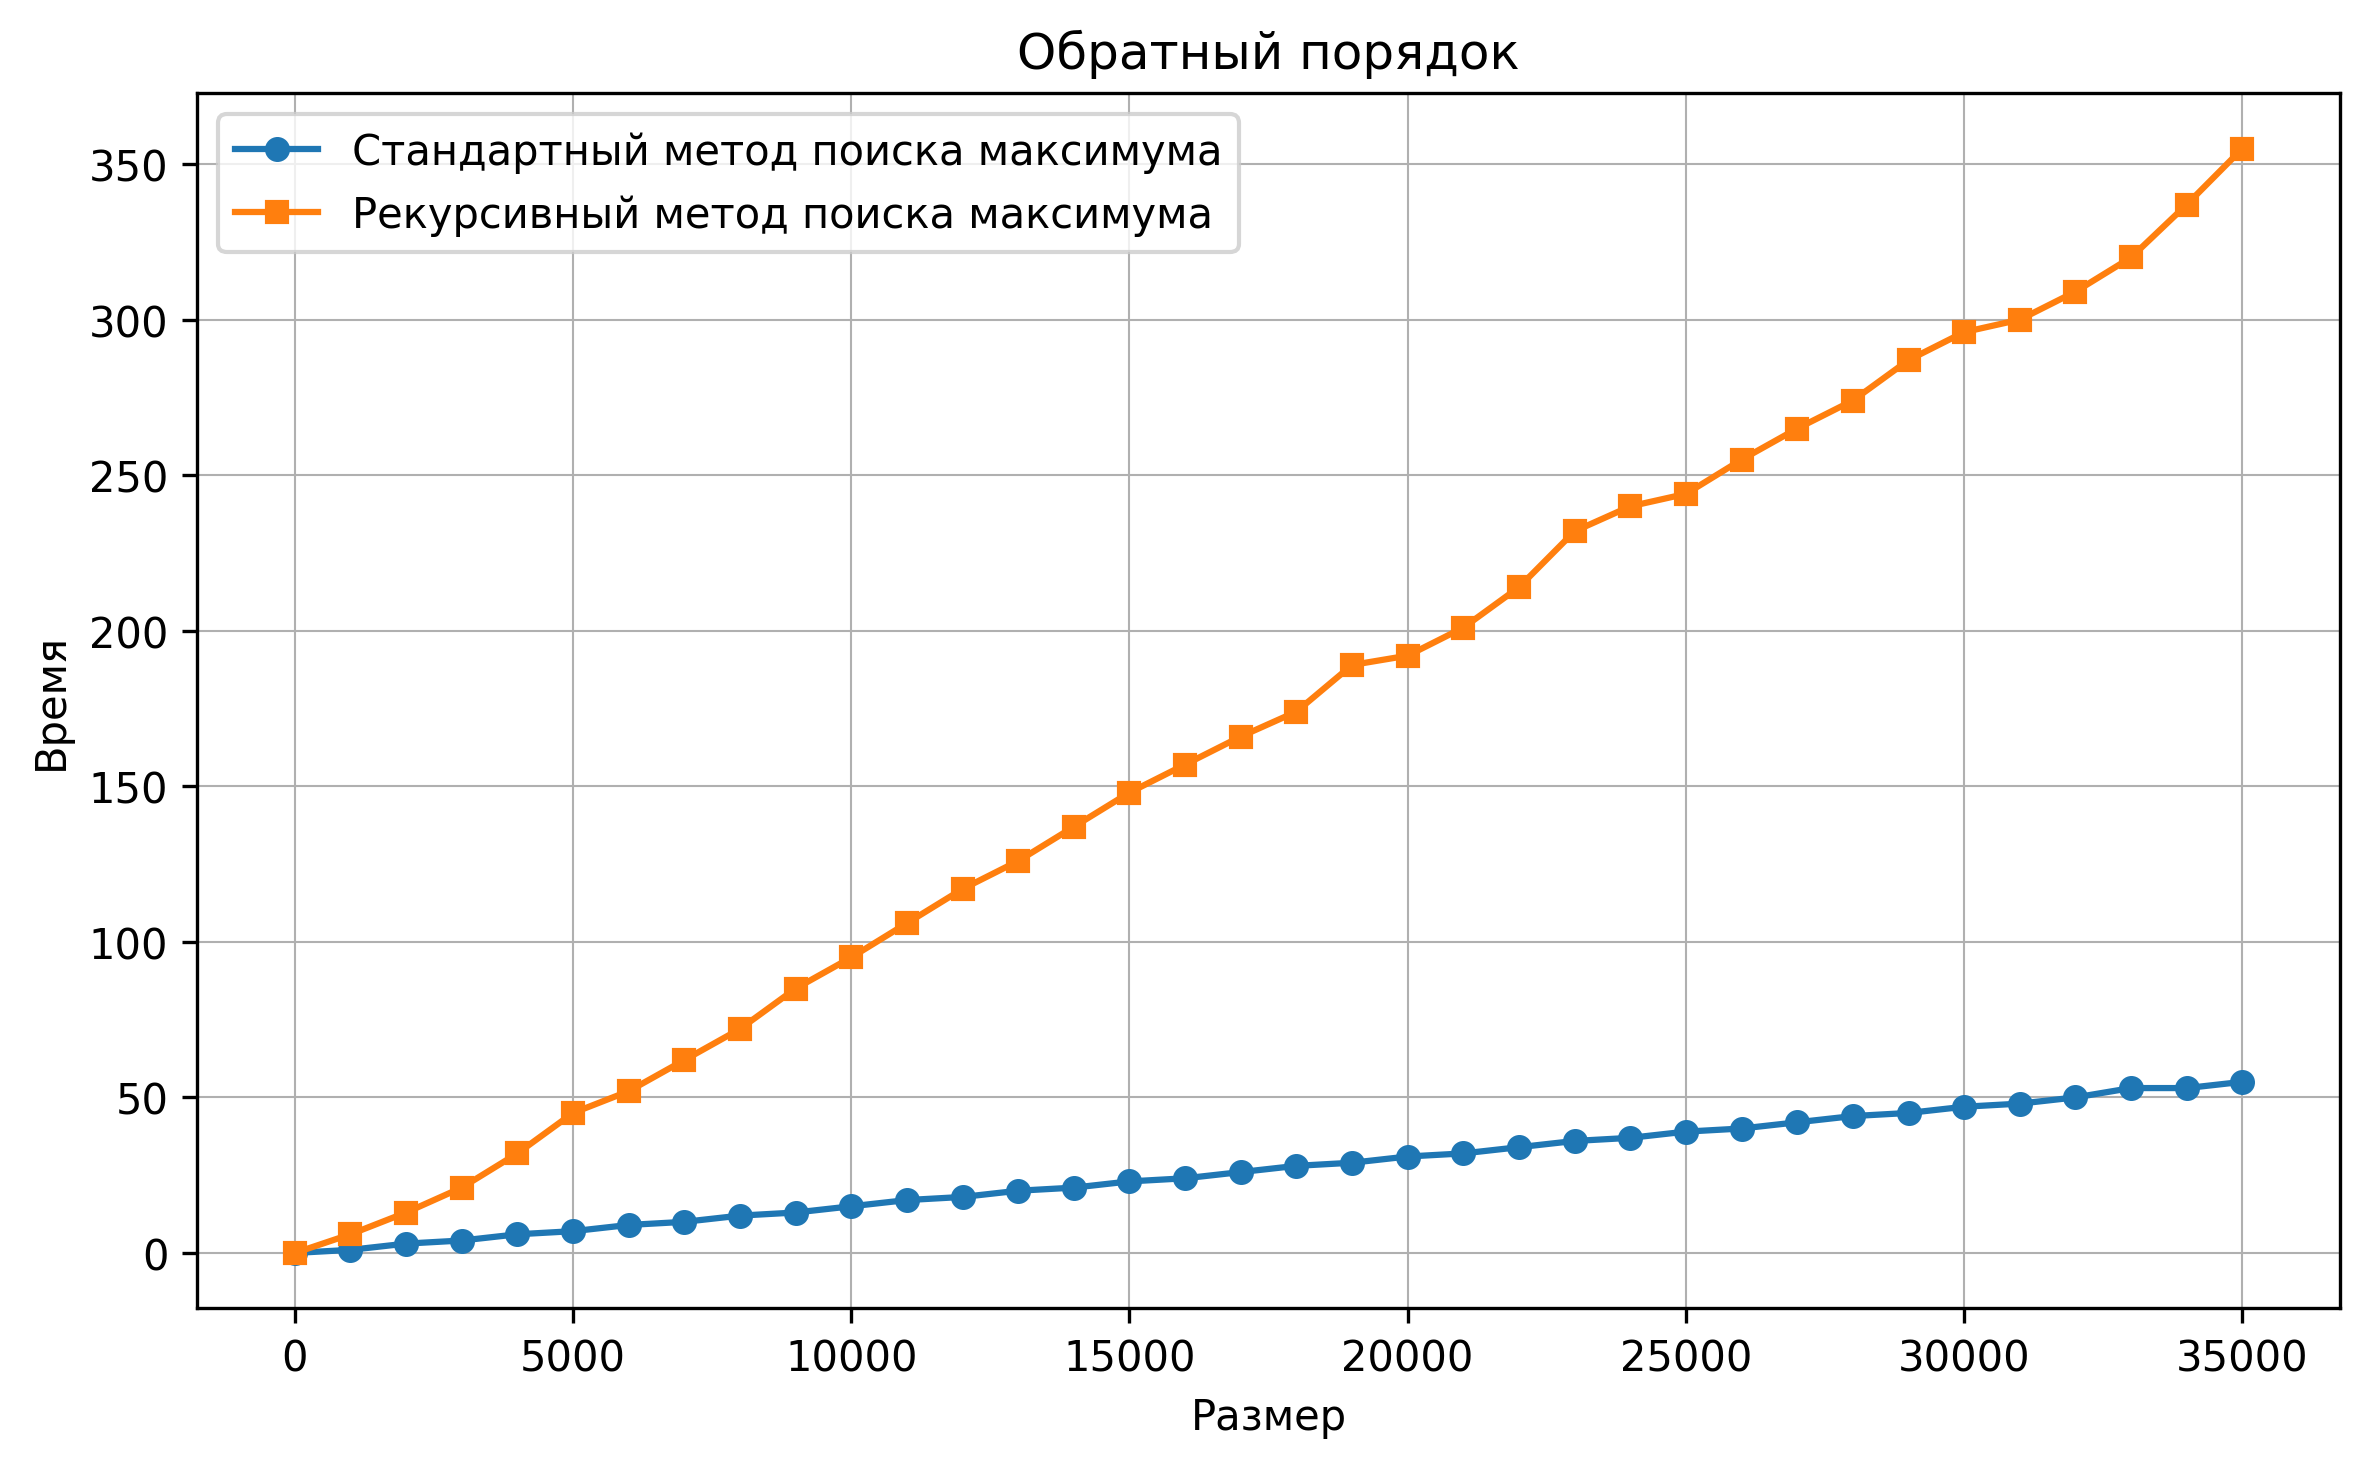
\includegraphics[width=0.9\linewidth]{./images/chart_2.png}
	\caption{Зависимость времени выполнения реализации алгоритма от размера массива, заполненного числами в порядки убывания}
	\label{fig:reverse}
\end{figure}


\section*{Вывод}
реализации исследовательской части было выяснено, что итерационный алгоритм поиска максимально элемента массива выполняется быстрее в 7 раз в лучшем случае и в 4 раза в худшем случае чем рекурсивный алгоритм. Была установлена зависимость времени выполнения от сортировки входных данных. Выяснено, что поиск максимального элемента в массиве отсортированном м в порядке убывания оказался быстрее на 20\% чем поиск в массиве отсортированном в порядке возрастания.

\clearpage
